\documentclass[12pt,a4paper,oneside]{article}

\usepackage[QX]{polski}

\usepackage[utf8]{inputenc}
\usepackage{latexsym}
\usepackage{tgpagella}
\usepackage{lmodern}
\usepackage{amsmath,amsthm,amsfonts,amssymb,alltt}
\usepackage{epsfig}
\usepackage{pdflscape}
\usepackage{caption}
\usepackage{indentfirst}
\usepackage{float}
%\usepackage{showkeys}
\bibliographystyle{plabbrv}
\usepackage[utf8]{inputenc}
\usepackage{listings}
\usepackage{xcolor}
\usepackage{color}
\usepackage[polish]{babel}
\usepackage{datetime2}
\usepackage[x11names,dvipsnames,table]{xcolor}
\usepackage{hyperref}
\usepackage{tabularx}

\usepackage{adjustbox}

\hypersetup{
pdfauthor={Roman Czapla, Olaf Bar},
colorlinks=True,
linkcolor=darkgray,  % color of internal links (change box color with linkbordercolor)
citecolor=BrickRed,  % color of links to bibliography
filecolor=Magenta,   % color of file links
urlcolor=BlueViolet}	%%pdfpagemode=FullScreen}

% diagramy, grafy itp.
\usepackage{tikz}
\usetikzlibrary{positioning}
\usetikzlibrary{arrows}
\usetikzlibrary{arrows.meta}
\usetikzlibrary{chains,fit,shapes,calc}
\tikzset{main node/.style={circle,fill=blue!20,draw,minimum size=1cm,inner sep=0pt}}

% algorytmy
\usepackage[linesnumbered,lined,commentsnumbered]{algorithm2e}
\SetKwFor{ForEach}{for each}{do}{end for}%
\SetKwFor{ForAll}{for all}{do}{end for}%
\newenvironment{myalgorithm}
{\rule{\textwidth}{0.5mm}\\\SetAlCapSty{}\SetAlgoNoEnd\SetAlgoNoLine\begin{algorithm}}{\end{algorithm}\rule{\textwidth}{0.5mm}}


%---------------------

\pagestyle{plain}
\textwidth=15cm \textheight=685pt \topmargin=-25pt \linespread{1.3} 
\setlength{\parskip}{0pt}
\setlength\arraycolsep{2pt}
\oddsidemargin = 0.9cm
\evensidemargin =-0.1cm

\captionsetup{width=.95\linewidth, justification=centering}
%---------------------

\newtheorem{tw}{Twierdzenie}[section]
\newtheorem{lem}[tw]{Lemat}
\newtheorem{co}[tw]{Wniosek}
\newtheorem{prop}[tw]{Stwierdzenie}
\theoremstyle{definition}
\newtheorem{ex}{Przykład}
\newtheorem{re}[tw]{Uwaga}
\newtheorem{de}{Definicja}[section]



\newcommand{\bC}{{\mathbb C}}
\newcommand{\bR}{{\mathbb R}}
\newcommand{\bZ}{{\mathbb Z}}
\newcommand{\bQ}{{\mathbb Q}}
\newcommand{\bN}{{\mathbb N}}
\newcommand{\captionT}[1]{\caption{\textsc{\footnotesize{#1}}}}
\renewcommand\figurename{Rys.}

\numberwithin{equation}{section}
\renewcommand{\thefootnote}{\arabic{footnote})}
%\renewcommand{\thefootnote}{\alph{footnote})}


% Definiowanie kolorów dla kodu źródłowego
\definecolor{codegreen}{rgb}{0,0.6,0}
\definecolor{codegray}{rgb}{0.5,0.5,0.5}
\definecolor{codepurple}{rgb}{0.58,0,0.82}
\definecolor{backcolour}{rgb}{0.95,0.95,0.92}

% Ustawienia wyglądu kodu źródłowego
\lstdefinestyle{mystyle}{
    backgroundcolor=\color{backcolour},   
    commentstyle=\color{codegreen},
    keywordstyle=\color{magenta},
    numberstyle=\tiny\color{codegray},
    stringstyle=\color{codepurple},
    basicstyle=\ttfamily\footnotesize,
    breakatwhitespace=false,         
    breaklines=true,                 
    captionpos=b,                    
    keepspaces=true,                 
    numbers=left,                    
    numbersep=5pt,                  
    showspaces=false,                
    showstringspaces=false,
    showtabs=false,                  
    tabsize=2
}




\begin{document}

% --------------------------------------------
% Strona tytułowa
% --------------------------------------------

\thispagestyle{empty}
\begin{titlepage}
\begin{center}\Large
Uniwersytet Komisji Edukacji Narodowej w Krakowie\\
\large
Instytut Bezpieczeństwa i Informatyki\\
\vskip 10pt
\end{center}
\begin{center}
\centering 
\includegraphics[width=1.0\columnwidth]{images/logo.png}
\end{center}

\begin{center}
 {\bf \fontsize{14pt}{14pt}\selectfont PROJEKT INŻYNIERSKI\\ DOKUMENTACJA PROJEKTOWA}
\end{center}
\vskip 5pt
\begin{center}
 {\bf \fontsize{22pt}{22pt}\selectfont RADAR ODCINKOWY}
\end{center}

\begin{center}
 {\fontsize{12pt}{12pt}\selectfont wykonany przez: }
\end{center}
\begin{center}
 {\bf\fontsize{16pt}{16pt}\selectfont Tomasz Górski}\\
 {\fontsize{12pt}{12pt}\selectfont Nr albumu: 151896 \\\&\\}
 {\bf\fontsize{16pt}{16pt}\selectfont Tomasz Joniec}\\
 {\fontsize{12pt}{12pt}\selectfont Nr albumu: 151861\\\&\\}
 {\bf\fontsize{16pt}{16pt}\selectfont Patryk Golonka}\\
 {\fontsize{12pt}{12pt}\selectfont Nr albumu: 145857}
\end{center}
\begin{center}
 {\fontsize{12pt}{12pt}\selectfont pod opieką:}\\
 {\bf\fontsize{12pt}{12pt}\selectfont dr inż. Grzegorz Sokal, mgr Łukasz Przybytek}
\end{center}

%\mbox{}
\vspace*{\fill}
%\vskip 50pt
\begin{center}
\large
Kraków \the\year\\
(ostatnia aktualizacja: \DTMcurrenttime,\;\today)
\end{center}
\end{titlepage}
\setcounter{page}{0} 
\newpage\null\thispagestyle{empty}
%\setcounter{page}{0} 
%\newpage
%\thispagestyle{empty}

\tableofcontents


\newpage

\section{Szczegółowa dokumentacja projektowa}
\subsection{Projekt UML}
        \begin{figure}[H]
          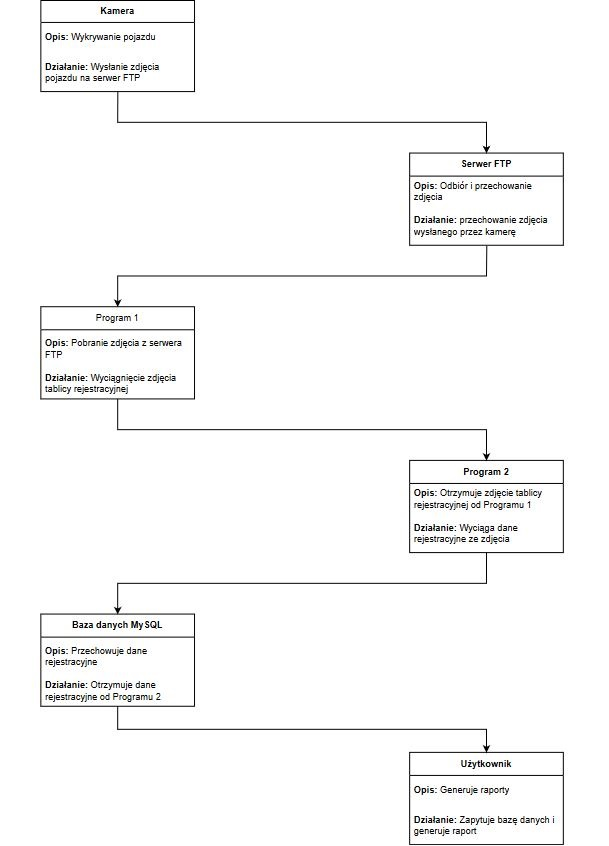
\includegraphics[width=0.8\linewidth]{dokumentacja_projektowa/images/uml.JPG}
          \label{fig:Generowanie}
        \end{figure}

        \newpage
\subsection{Projekt bazy danych}
Baza danych 'radar' składa się z 4 tabel, które służą do zbierania danych wejściowych z kamer oraz do prezentowania wyników za pomocą raportu dla zarejestrowanych użytkowników. Poniżej opis tabel wraz z omówieniem kolumn przechowujących dane.\\

    Tabela cars zawiera 10 pól:
    \begin{table}[h]
    \centering
    \begin{tabularx}{\textwidth}{|X|X|X|}
    \hline
    \textbf{Nazwa} & \textbf{Opis} \\ \hline
    id &  -   \\ \hline
    brand & marka \\  \hline
    model & - \\  \hline
    year{\_}of{\_}manufacture & rok produkcji \\  \hline
    first{\_}registration{\_}date & data pierwszej rejestracji \\  \hline
    color & - \\  \hline
    plate{\_}number & numer rejestracyjny \\ \hline
    owner{\_}name & nazwa właściciela \\ \hline
    owner{\_}address & adres właściciela \\ \hline
    owner{\_}contact{\_}number & numer kontaktowy właściciela\\ \hline
    \end{tabularx}
    \caption{Tabela cars}
    \end{table}
        
        Tabela przechowuje szczegółowe informacje o samochodach, w tym ich markę, model, kolor oraz dane właściciela. W środowisku produkcyjnym tabela ta musiałaby posiadać informacje o wszystkich samochodach zajerejestrowanych w Polsce oraz ich włascicielach, ponieważ bez tych danych byłoby niemożliwe wygenerowanie raportu ze zdarzenia z poziomu aplikacji webowej. Dane w tej tabeli mogłby replikować się z rządowych baz danych.  

    \newpage
    Tabela plates zawiera 9 pól:

    \begin{table}[h]
    \centering
    \begin{tabularx}{\textwidth}{|X|X|X|}
    \hline
    \textbf{Nazwa} & \textbf{Opis} \\ \hline
    id &  -   \\ \hline
    timestamp{\_}in & czas rozpoczęcia pomiaru \\  \hline
    location{\_}in & lokalizacja rozpoczęcia pomiaru \\  \hline
    plate{\_}number{\_}in & numer rejestracyjny przy starcie pomiaru \\  \hline
    timestamp{\_}out & czas zakończenia pomiaru \\  \hline
    location{\_}out & lokalizacja zakończenias pomiaru \\ \hline
    plate{\_}number & numer rejestracyjny \\ \hline
    plate{\_}number{\_}out & numer tablicy przy zakończeniu pomiaru \\ \hline
    isDeleted & flaga usuniętego rekordu \\ \hline
    \end{tabularx}
    \caption{Tabela plates}
    \end{table}
        
        Tabela używana do śledzenia wejścia i wyjścia pojazdów z ich numerami tablic w określonych miejscach i czasach. Jest kluczowa z punktu widzenia systemu radaru odcinkowego, ponieważ zbiera informacje o wykroczeniach prędkości i na jej podstawie analizowana jest prędkość średnia na wybranym odcinku drogi.\\


    Tabela raport zawiera 5 pól: 

    \begin{table}[h]
    \centering
    \begin{tabularx}{\textwidth}{|X|X|X|}
    \hline
    \textbf{Nazwa} & \textbf{Opis} \\ \hline
    id &  -   \\ \hline
    timestamp{\_}in & czas wygenerowania raportu \\  \hline
    speed & prędkość \\  \hline
    plates{\_}id & identyfikator rekordu tablicy rejestracyjnej \\  \hline
    \end{tabularx}
    \caption{Tabela raport}
    \end{table}
            
        Tabela używana do celów raportowania, zawiera informacje o wygenerowanym raporcie, przechowuje prędkość na zmierzonym odcinku oraz wysokość należnego mandatu wraz z kluczem obcym do tabeli plates.

    \newpage
    Tabela users zawiera 3 pola:

    \begin{table}[h]
    \centering
    \begin{tabularx}{\textwidth}{|X|X|X|}
    \hline
    \textbf{Nazwa} & \textbf{Opis} \\ \hline
    id &  -   \\ \hline
    username{\_}in & nazwa użytkownika \\  \hline
    password & hasło \\  \hline
    \end{tabularx}
    \caption{Tabela users}
    \end{table}

       Tabela służy do przechowywania poświadczeń użytkowników z unikanymi nazwami oraz powiązanymi hasłami z procesu rejestracji konta. Na cele projektowe jest wystarczająca natomiast zostawia spore możliwości rozwoju, które powinny zostać wykorzystane podczas rozwiajanie funkcjonalości projektu. 




\subsection{Szczegółowa dokumentacja kodu}


Omówienie katalogu \textbf{cut{\_}plate{\_}from{\_}picture}. Katalog {cut{\_}plate{\_}from{\_}picture} zawiera plik licenseplate.py, którego działanie zostanie opisane poniżej.
\begin{enumerate}

\item Biblioteki oraz konfiguracja pytesseract 

\begin{adjustbox}{max width=\textwidth}
\begin{lstlisting}[language=Python]
    import cv2
    import pytesseract
    import numpy as np
    import os
    import re
    pytesseract.pytesseract.tesseract_cmd = '/usr/bin/tesseract'
\end{lstlisting}
\end{adjustbox}

 Ta sekcja importuje niezbędne biblioteki i konfiguruje Pytesseract, określając ścieżkę do wykonawczego pliku Tesseract. Te biblioteki są niezbędne do przetwarzania obrazów (OpenCV), OCR (Pytesseract), manipulacji tablicami (NumPy) oraz do operacji na plikach (os, re).


\item Ekstrakcja i formatowanie nazw plików

\begin{adjustbox}{max width=\textwidth}
\begin{lstlisting}[language=Python]
    filename_parts = os.path.basename(image_filename).split('_')
    timestamp = filename_parts[0]
    additional_text = filename_parts[1].split('.')[0]
\end{lstlisting} 
\end{adjustbox}

Program ekstrahuje informacje z nazwy pliku obrazu. Ta część kodu jest odpowiedzialna za rozdzielanie nazwy pliku na komponenty, aby uzyskać znacznik czasu i dodatkowy tekst, które mogą być używane do dalszego przetwarzania lub nazywania plików wyjściowych.


\item Funkcja przetwarzania obrazu - process{\_}image(image{\_}filename)


To serce skryptu, gdzie odbywa się przetwarzanie obrazu i OCR.

\begin{adjustbox}{max width=\textwidth}
\begin{lstlisting}[language=Python]
    def process_image(image_filename):
        img = cv2.imread(image_filename)
        imgray1 = cv2.cvtColor(img, cv2.COLOR_BGR2GRAY)
        canny = cv2.Canny(imgray1, 313, 480)
        contours, _ = cv2.findContours(canny, cv2.RETR_TREE, cv2.CHAIN_APPROX_NONE)
\end{lstlisting}
\end{adjustbox}

Skrypt odczytuje obraz, konwertuje go na odcienie szarości i używa detektora krawędzi Canny do znalezienia krawędzi. Następnie pobiera kontury z obrazu, priorytetyzując je według wielkości.

\item Przetwarzanie konturów i izolacja tablic rejestracyjnych

\begin{adjustbox}{max width=\textwidth}
\begin{lstlisting}[language=Python]
    for i in contours:
        area = cv2.contourArea(i)
        approx = cv2.approxPolyDP(i, 0.01*cv2.arcLength(i, True), True)
        if len(approx) == 4 and area > 800:
            cv2.drawContours(img, [approx], 0, (0, 255, 0), 2)
            x, y, w, h = cv2.boundingRect(i)
            img4 = imgray1[y:y+h, x:x+w]
\end{lstlisting}    
\end{adjustbox}

Iteruje przez kontury, aby znaleźć czworokąt (prawdopodobnie tablicę rejestracyjną) na podstawie jego kształtu i wielkości. Gdy prawdopodobny kandydat zostanie znaleziony, wyodrębnia tę część obrazu do OCR.

\item Ekstrakcja tekstu OCR

\begin{adjustbox}{max width=\textwidth}
\begin{lstlisting}[language=Python]
    try:
        license_plate = pytesseract.
        image_to_string(img4, config='--psm 7')
    except:
        print("Nie mozna odczytac 
        tablicy rejestracyjnej.")
        return
\end{lstlisting} 
\end{adjustbox}



Używa Pytesseract do wstępnego odczytania tablicy rejestracyjnej. Jest to opcja która może zostać wykorzystana przy ewentualnej rozbudowie programu. Blok 'try-except' zapewnia, że program nie zakończy się awaryjnie, jeśli OCR nie uda się odczytać tekstu.

\item Post-processing i wyjście tekstu

\begin{adjustbox}{max width=\textwidth}
\begin{lstlisting}[language=Python]
    plate_number_raw = pytesseract.image_to_string(morph_img, config='--psm 8 --oem 3')
    plate_number = plate_number_raw.replace(':', '').strip()
    print("Extracted Plate Number:", plate_number)
\end{lstlisting} 
\end{adjustbox}


Po OCR skrypt wykonuje pewne czyszczenie wyekstrahowanego tekstu, usuwając niechciane znaki i przycinając białe znaki, a następnie wyświetla oczyszczony numer tablicy.




\item Zapisywanie i obsługa plików

\begin{adjustbox}{max width=\textwidth}
\begin{lstlisting}[language=Python]
    cv2.imwrite('workdir/only_plate.jpg', img4)
    ...
    cv2.imwrite(full_save_path, white_canvas)
    ...
    if os.path.exists(work_directory):
        for filename in os.listdir(work_directory):
            os.unlink(work_path)
\end{lstlisting} 
\end{adjustbox}


Skrypt zapisuje średnie i końcowe przetworzone obrazy do przeglądu lub dalszego użytku. Docelowe pliki są zostają zapisane w podfolderze images. Skrypt również kod do czyszczenia miejsca pracy przez usunięcie tymczasowych plików po przetwarzaniu w katalogu workdir.

\item Kontrola przetwarzania wsadowego

\begin{adjustbox}{max width=\textwidth}
\begin{lstlisting}[language=Python]
start_files = []
meta_files = []

for filename in os.listdir(directory):
    if filename.endswith(start + '.jpg'):
        start_files.append(filename)
    elif filename.endswith(meta + '.jpg'):
        meta_files.append(filename)

def process_files(file_list):
    for filename in file_list:
        file_path = os.path.join(directory, filename)
        process_image(file_path)

\end{lstlisting} 
\end{adjustbox}

Program segreguje pliki na podstawie ich nazw końcówek, tworząc odrębne listy dla różnych kategorii plików (tutaj jako przykład "balice" i "chrzanow"). Następnie używa funkcji process{\_}files do przetworzenia każdego zestawu plików. To organizuje przetwarzanie w bardziej zarządzalne i modularne grupy.

\item Wstępna obsługa plików graficznych

Dostarczony skrypt to rozwiązanie do przetwarzania wstępnego obrazów w celu ekstrakcji tablic rejestracyjnych z zidentyfikowanych pojazdów samochodowych. Łączy on techniki przetwarzania obrazów w celu przygotowania ich do OCR, a następnie używa Pytesseract do ekstrakcji tekstu natomiast głównym jego założeniem jest wydobycie rejestracji ze zdjęcia i przedstawienie jej jako grafiki na białym tle w celu dalszego przetwarzania. Skrypt jest zorganizowany tak, aby automatycznie obsługiwać wiele obrazów.
\end{enumerate}


\newpage






Następnym katalogiem do omówienia jest \textbf{find{\_}plate{\_}number}. W tym katalogu znajduje się kod odpowiedzialny za rozpoznanie numerów rejestracyjnych z obrazu przygotowanego przez kod z {cut{\_}plate{\_}from{\_}picture}. 

Katalog find{\_}plate{\_}number zawiera następujące elementy:

\begin{itemize}
  \item Skrypt główny main.py
  \item Plik wyników results.json
  \item Podkatalogi registration{\_}processing i resources
\end{itemize}



Podkatalog registration{\_}processing zawiera kluczowe skrypty do przetwarzania i rozpoznawania tablic rejestracyjnych. Podkatalog resources przechowuje obrazy liter i cyfr używane w procesie rozpoznawania.
Skrypt główny main.py koordynuje cały proces rozpoznawania tablic rejestracyjnych, włączając w to wczytywanie obrazów, ekstrakcję danych, rozpoznawanie numerów rejestracyjnych, oraz interakcje z bazą danych. Wykorzystuje moduły z `registration{\_}processing` do wykonania wybranych zadań.

Moduł registration{\_}processing zawiera dwa skrypty:

\begin{itemize}
  \item character{\_}classifier.py odpowiada za trenowanie klasyfikatora znaków i generowanie ich konturów.
  \item license{\_}plate{\_}recognizer.py zawiera logikę do rozpoznawania tablic rejestracyjnych, w tym przetwarzanie obrazów, wyszukiwanie potencjalnych tablic i znaków, a także końcowe rozpoznawanie i weryfikację tablic rejestracyjnych.
\end{itemize}

Opis character{\_}classifier.py

\begin{adjustbox}{max width=\textwidth}
\begin{lstlisting}[language=Python]
import numpy as np
import cv2
import glob
import re
import os

MIN_CONTOUR_AREA = 100
RESIZED_IMAGE_WIDTH = 20
RESIZED_IMAGE_HEIGHT = 30

\end{lstlisting} 
\end{adjustbox}

Ten fragment kodu rozpoczyna się od importowania potrzebnych bibliotek, takich jak numpy (do pracy z tablicami numerycznymi), cv2 (OpenCV do przetwarzania obrazów), glob (do wyszukiwania plików w określonym katalogu), re (do obsługi wyrażeń regularnych) i os (do operacji na systemie plików). Następnie definiowane są pewne stałe, takie jak minimalna powierzchnia konturu (MIN{\_}CONTOUR{\_}AREA) oraz szerokość i wysokość obrazu po przeskalowaniu (RESIZED{\_}IMAGE{\_}WIDTH i RESIZED{\_}IMAGE{\_}HEIGHT).

\begin{adjustbox}{max width=\textwidth}
\begin{lstlisting}[language=Python]
def get_chars_contour():
    images_dir = "resources/characters/"
    data_path = os.path.join(images_dir, '*g')
    files = glob.glob(data_path)

    chars_contour = {}

    for f1 in files:
        img_character = cv2.imread(f1, 0)
        letter = re.findall(r"q\w", f1)
        img_letter_edges = cv2.Canny(img_character, 30, 200)
        contours, hierarchy = cv2.findContours(img_letter_edges.copy(), cv2.RETR_EXTERNAL, cv2.CHAIN_APPROX_NONE)
        chars_contour[str(letter[0][1])] = contours

    return chars_contour
\end{lstlisting} 
\end{adjustbox}

Funkcja get{\_}chars{\_}contour służy do wczytywania obrazów znaków, przetwarzania ich w celu uzyskania konturów i zapisywania tych konturów w słowniku chars{\_}contour. Proces ten polega na:



\begin{itemize}
  \item Określeniu ścieżki do katalogu z obrazami znaków.
  \item Wyszukaniu wszystkich plików obrazów w katalogu.
  \item Iterowaniu przez każdy plik obrazu znaku.
  \item Wczytaniu obrazu, odczytaniu informacji o znaku z nazwy pliku, wygenerowaniu obrazu krawędzi znaku i znalezieniu jego konturu.
  \item Zapisaniu konturu znaku w słowniku, gdzie kluczem jest znak.
\end{itemize}

\begin{adjustbox}{max width=\textwidth}
\begin{lstlisting}[language=Python]
def train_classifier(chars{\_}contour):
    img_training_chars = cv2.imread("resources/all{\_}characters.jpg")
    if img_training{\_}chars is None:
        print("blad nie mozna odczytac pliku. Sprawdz sciezke pliku")
        os.system("pause")
        return

    img_gray = cv2.cvtColor(img_training_chars, cv2.COLOR_BGR2GRAY)

    ret, img_thresh = cv2.threshold(img_gray, 150, 255, cv2.THRESH_BINARY_INV)
    img_thresh_copy = img_thresh.copy()

    npa_contours, npa_hierachy = cv2.findContours(img_thresh_copy,
                                                  cv2.RETR_EXTERNAL,
                                                  cv2.CHAIN_APPROX_SIMPLE)

    npa_flattened_images = np.empty((0, RESIZED_IMAGE_WIDTH*RESIZED_IMAGE_HEIGHT))
    int_classifications = []

    for idx, npa_contour in enumerate(npa_contours):
        if cv2.contourArea(npa_contour) > MIN_CONTOUR_AREA:
            [intX, intY, intW, intH] = cv2.boundingRect(npa_contour)

            img_ROI = img_thresh[intY-5:intY+intH+5, intX-5:intX+intW+5]
            img_ROI1 = img_thresh[intY:intY+intH, intX:intX+intW]
            img_ROI_resized = cv2.resize(img_ROI1, (RESIZED_IMAGE_WIDTH, RESIZED_IMAGE_HEIGHT))

            img_ROI_edges = cv2.Canny(img_ROI.copy(), 30, 200)

            contours_ROI, hierarchy_ROI = cv2.findContours(img_ROI_edges.copy(),
                                                           cv2.RETR_EXTERNAL, cv2.CHAIN_APPROX_NONE)
            matches = {}
            for letter, letter_cntr in chars_contour.items():
                ret = cv2.matchShapes(letter_cntr[0], contours_ROI[0], 1, 0.0)
                matches[letter] = ret
            best = min(matches, key=matches.get)
            
            if idx == 0 and best == '6':
                best = '9'
            if idx == 7 and best == 'S':
                best = '2'
            if idx == 10 and best == 'O':
                best = 'M'
            if idx == 11 and best == 'O':
                best = "N"
            if idx == 15 and best == 'O':
                best = 'X'
            if idx == 23 and best == '0':
                best = 'D'
            if idx == 30 and best == 'O':
                best = 'W'
            int_classifications.append(ord(best))
            npa_flattened_image = img_ROI_resized.reshape((1, RESIZED_IMAGE_WIDTH * RESIZED_IMAGE_HEIGHT))
            npa_flattened_images = np.append(npa_flattened_images, npa_flattened_image, 0)

    flt_classifications = np.array(int_classifications, np.float32)
    npa_classifications = flt_classifications.reshape((flt_classifications.size, 1))
    return npa_classifications, npa_flattened_images
\end{lstlisting} 
\end{adjustbox}

   Funkcja train{\_}classifier służy do przetwarzania obrazu treningowego zawierającego wiele znaków, wyodrębniania poszczególnych znaków, dopasowywania ich do wcześniej zdefiniowanych konturów znaków i tworzenia zestawu spłaszczonych obrazów znaków wraz z odpowiadającymi im klasyfikacjami. Metoda została dostosowana z repozytorium github.com: OpenCV{\_}3{\_}KNN{\_}Character{\_}Recognition{\_}Python.



Proces ten obejmuje:
\begin{itemize}
  \item Wczytanie obrazu treningowego zawierającego wszystkie znaki.
  \item Konwersję obrazu na odcienie szarości.
  \item Progowanie obrazu.
  \item Znajdowanie konturów dla wszystkich znaków na obrazie.
  \item Przygotowanie pustej tablicy numpy (npa{\_}flattened{\_}images) do przechowywania spłaszczonych obrazów znaków.
  \item  Przygotowanie pustej listy (int{\_}classifications) do przechowywania klasyfikacji znaków.
\end{itemize}
    

Dodatkowo dla każdego konturu znaku:
\begin{itemize}
  \item Sprawdzenie, czy kontur jest wystarczająco duży.
  \item Wyodrębnienie obszaru zainteresowania (ROI) wokół konturu.
  \item Dopasowanie konturu ROI do znaków treningowych i wybór najlepszego dopasowania.
  \item Dodanie klasyfikacji znaku do listy int{\_}classifications jako kod Unicode.
  \item Spłaszczenie obrazu ROI i dodanie go do npa{\_}attened{\_}images.

\end{itemize}

Na końcu funkcja zwraca tablicę numpy npa{\_}classifications zawierającą klasyfikacje znaków oraz npa{\_}flattened{\_}images zawierającą spłaszczone obrazy znaków.    
    
Opis license{\_}plate{\_}recognizer.py

\begin{adjustbox}{max width=\textwidth}
\begin{lstlisting}[language=Python]
import numpy as np
import cv2
kNearest = cv2.ml.KNearest_create()
PLATE_HEIGHT_TO_WIDTH_RATIO = 90 / 520
CHAR_RATIO_MIN = 0.25
CHAR_RATIO_MAX = 0.85
LICENSE_PLATE_LENGTH = 7
RESIZED_CHAR_IMAGE_WIDTH = 20
RESIZED_CHAR_IMAGE_HEIGHT = 30
SHOW_STEPS = False

\end{lstlisting} 
\end{adjustbox}

Główna funkcja recognize{\_}license{\_}plate koordynuje cały proces rozpoznawania tablicy rejestracyjnej, od przetwarzania wstępnego po końcową weryfikację i rozpoznawanie znaków. Stałe zdefiniowane w skrypcie license{\_}plate{\_}recognizer.py są kluczowymi wartościami, które sterują różnymi aspektami procesu rozpoznawania tablic rejestracyjnych. Oto ich szczegółowy opis:

\begin{itemize}
  \item PLATE{\_}HEIGHT{\_}TO{\_}WIDTH{\_}RATIO - określa stosunek wysokości do szerokości typowej polskiej tablicy rejestracyjnej. W Polsce standardowy wymiar tablicy to 520 mm szerokości na 114 mm wysokości, co daje stosunek około 0,2192 (114/520). Jest to używane do identyfikowania potencjalnych tablic rejestracyjnych na obrazie poprzez porównywanie wymiarów znalezionych konturów z tym stosunkiem.
  \item CHAR{\_}RATIO{\_}MIN i CHAR{\_}RATIO{\_}MAX - Określają minimalny i maksymalny akceptowalny stosunek wysokości do szerokości pojedynczego znaku na tablicy rejestracyjnej. Te proporcje są wykorzystywane do filtrowania potencjalnych znaków na podstawie ich geometrycznych cech, eliminując te, które nie pasują do typowych rozmiarów liter i cyfr.
  \item LICENSE{\_}PLATE{\_}LENGTH - Oznacza oczekiwaną liczbę znaków na polskiej tablicy rejestracyjnej, która wynosi 7. Jest to kluczowe dla procesu weryfikacji i finalizacji rozpoznawania tablicy rejestracyjnej, aby upewnić się, że ostateczny wynik zawiera odpowiednią liczbę znaków.
  \item RESIZED{\_}CHAR{\_}IMAGE{\_}WIDTH i RESIZED{\_}CHAR{\_}IMAGE{\_}HEIGHT - to wymiary (szerokość i wysokość), do których każdy potencjalny znak jest skalowany przed przetwarzaniem przez klasyfikator (np. KNN). Jednolite rozmiary są ważne dla spójności danych wejściowych do modelu klasyfikacji. W przypadku tego skryptu wymiary te wynoszą odpowiednio 20 i 30 pikseli.
  \item SHOW{\_}STEPS - jest to zmienna logiczna (prawda/fałsz), która kontroluje, czy skrypt powinien wyświetlać poszczególne kroki i wyniki pośrednie procesu rozpoznawania tablic rejestracyjnych (np. wyświetlanie obrazów w trakcie przetwarzania). Ustawienie jej na True umożliwia wizualizację i debugowanie procesu, podczas gdy False prowadzi do cichszego wykonania bez wyświetlania dodatkowych informacji.
\end{itemize}

\begin{adjustbox}{max width=\textwidth}
\begin{lstlisting}[language=Python]
def train_KNN(classifications, flattened_images):
    npa_classifications = classifications.astype(np.float32)
    npa_flattened_images = flattened_images.astype(np.float32)
    npa_classifications = npa_classifications.reshape((npa_classifications.size, 1))
    kNearest.setDefaultK(1)
    kNearest.train(npa_flattened_images, cv2.ml.ROW_SAMPLE, npa_classifications)
    return True
\end{lstlisting} 
\end{adjustbox}

Funkcja `train\_KNN` służy do trenowania klasyfikatora k-Nearest Neighbors (k-NN) używanego do rozpoznawania znaków na tablicach rejestracyjnych. 
Konwersja typów danych:
\begin{itemize}
  \item **classifications** i **flattened\_images** są konwertowane na typ `np.float32`. Jest to standardowa praktyka w uczeniu maszynowym, ponieważ wiele algorytmów działa lepiej lub wymaga danych zmiennoprzecinkowych.
  \item **classifications** to tablica zawierająca etykiety klas (np. której litery czy cyfry odpowiada dany obraz).
  \item **flattened\_images** to spłaszczone obrazy znaków, które są używane jako dane wejściowe dla klasyfikatora. Spłaszczenie polega na przekształceniu obrazu z dwuwymiarowej matrycy pikseli na jednowymiarowy wektor.
\end{itemize}





Przekształcenie klasyfikacji - npa\_classifications jest przekształcana tak, aby miała wymiary (`n`, 1), gdzie `n` to liczba próbek. Jest to konieczne, ponieważ OpenCV oczekuje, że etykiety klas będą w tej formie.

Ustawienie parametru 'K' dla k-NN - kNearest.setDefaultK(1) ustawia parametr K klasyfikatora k-NN na 1. Oznacza to, że klasyfikacja danej próbki będzie oparta na najbliższym sąsiedzie w przestrzeni cech.

Trenowanie klasyfikatora - metoda `train` klasyfikatora k-NN jest wywoływana z `npa\_flattened\_images` jako danymi treningowymi i `npa\_classifications` jako etykietami. Parametr `cv2.ml.ROW\_SAMPLE` informuje klasyfikator, że każdy wiersz `npa\_flattened\_images` stanowi osobną próbkę.


Zwracanie wyniku -funkcja zwraca `True`, sygnalizując pomyślne zakończenie procesu trenowania.

Opis pozostałych fukcji z pliku license{\_}plate{\_}recognizer.py:
\begin{enumerate}
  \item get{\_}potential{\_}chars{\_}ROI: Szuka potencjalnych regionów zawierających znaki na tablicach rejestracyjnych.
  \item recognize{\_}chars{\_}in{\_}plate: Rozpoznaje znaki na tablicach rejestracyjnych na podstawie ROI.
  \item license{\_}plate{\_}rules: Sprawdza, czy rozpoznane tablice rejestracyjne pasują do polskich standardów tablic rejestracyjnych.
  \item preprocess: Przygotowuje obraz do dalszego przetwarzania poprzez skalowanie, rozmycie i wykrywanie krawędzi.
  \item find{\_}potential{\_}plates{\_}vertices: Szuka potencjalnych tablic rejestracyjnych na obrazie.
  \item get{\_}birds{\_}eye{\_}view: Zmienia perspektywę potencjalnych tablic rejestracyjnych na widok z góry.
  \item find{\_}potential{\_}chars{\_}on{\_}plates: Wyszukuje potencjalne znaki na tablicach rejestracyjnych.
  \item three{\_}chars{\_}in{\_}first{\_}part: Sprawdza, czy na tablicy rejestracyjnej są trzy znaki w pierwszej części.
  \item recognize{\_}license{\_}plate: Główna funkcja do rozpoznawania tablic rejestracyjnych na obrazach.
\end{enumerate}


Opis main.py

Skrypt main.py w projekcie rozpoznawania tablic rejestracyjnych pełni funkcję koordynatora całego procesu rozpoznania numerów rejestracyjnych pojazdów. Przeanalizujmy szczegółowo jego działanie i strukturę:
\begin{enumerate}

\item Importowanie Bibliotek

    Skrypt rozpoczyna się od importowania niezbędnych bibliotek i modułów, takich jak argparse, json, pathlib, re, cv2 (dla operacji na obrazach), mysql.connector (do obsługi bazy danych) oraz funkcji z modułu registration{\_}processing.

\item Funkcje Pomocnicze

    extract{\_}timestamp{\_}from{\_}filename: Wyodrębnia datę i czas z nazw plików.
    insert{\_}into{\_}database{\_}start i update{\_}database{\_}meta: Odpowiadają za komunikację z bazą danych MySQL, wstawiając i aktualizując rekordy dotyczące rozpoznanych tablic rejestracyjnych.

\item Przetwarzanie Obrazów

    process{\_}images: Ta funkcja przetwarza listę obrazów, używając recognize{\_}license{\_}plate do identyfikacji numerów rejestracyjnych. Wyniki są przechowywane w słowniku.


\item Główna funkcja main:

\begin{itemize}
  \item Parsowanie Argumentów \\
  Skrypt akceptuje argumenty dotyczące lokalizacji obrazów i pliku wynikowego.
  \item Przygotowanie Danych \\
  Obrazy są sortowane i przetwarzane w zależności od ich lokalizacji (np. Balice, Chrzanów).
  \item Trening Klasyfikatora \\
  Wywołuje funkcje get{\_}chars{\_}contour, train{\_}classifier, i train{\_}KNN do przygotowania modelu do rozpoznawania znaków.
  \item Rozpoznawanie Tablic Rejestracyjnych \\
  Skrypt przetwarza obrazy, rozpoznaje tablice rejestracyjne i zapisuje wyniki do pliku JSON
  \item Interakcja z Bazą Danych \\
  Wyniki są następnie przekazywane do funkcji zarządzających bazą danych.
\end{itemize}

    

\item Wykonywanie Skryptu

    Instrukcja if {\_}{\_}name{\_}{\_} == '{\_}{\_}main{\_}{\_}': zapewnia, że skrypt main.py działa jako główny program, kiedy jest uruchamiany bezpośrednio, a nie jako moduł importowany do innego skryptu.
\end{enumerate}

Skrypt main.py jest sercem systemu i koordynuje wszystkie kluczowe etapy procesu rozpoznawania tablic rejestracyjnych. Od wczytywania obrazów, poprzez ich analizę, rozpoznawanie znaków, aż po zapis wyników i interakcję z bazą danych. Jest to dobrze zorganizowany i modułowy kod, który efektywnie integruje różne aspekty systemu rozpoznawania tablic rejestracyjnych.



Katalog apache odpowiedzialny za serwis apache2 składa się z następujących plików i katalogów:

\begin{itemize}
  \item auth{\_}check.php \\
Skrypt odpowiedzialny za weryfikację, czy użytkownik jest zalogowany. Jest wykorzystywany w innych skryptach do sprawdzenia, czy użytkownik ma dostęp do określonych stron lub funkcji.  
  \item delete{\_}record.php \\
Skrypt do usuwania rekordów z bazy danych. Zamiast usuwania rekordu całkowicie, zmienia on flagę isDeleted na 1, co oznacza tzw. "miękkie usunięcie". Umożliwia to zachowanie danych dla celów archiwizacyjnych.  
  \item generate{\_}report.php \\
Skrypt generuje raport na podstawie wybranego rekordu. Pobiera dane z bazy, oblicza prędkość na podstawie czasu i lokalizacji, a następnie tworzy raport w formacie PDF, który jest następnie przekazywany do użytkownika do pobrania.  
  \item index.php \\
Ten plik wyświetla interfejs użytkownika dla strony głównej. Zawiera tabelę z rekordami dotyczącymi przypadków przekroczenia prędkości, włączając informacje takie jak ID, czas wejścia i wyjścia, lokalizację oraz numer rejestracyjny pojazdu. Użytkownicy mogą generować raporty lub usuwać rekordy.
  \item login.php \\
Skrypt logowania do systemu. Użytkownicy wpisują swoje dane (nazwę użytkownika i hasło), które są weryfikowane z bazą danych. W przypadku pomyślnego zalogowania użytkownik jest przekierowywany do strony głównej.
  \item logut.php \\
Ten plik służy do wylogowywania użytkowników. Usuwa wszystkie zmienne sesyjne i niszczy sesję, a następnie przekierowuje użytkownika do strony logowania.  
  
  \item registration.php \\
Skrypt obsługujący proces rejestracji nowych użytkowników. Umożliwia wprowadzenie nazwy użytkownika oraz hasła (i jego potwierdzenia), a następnie zapisuje te dane w bazie danych.  
  \item TCPDF
\end{itemize}
Katalog tcpdf to zewnętrzna biblioteka PHP służąca do generowania dokumentów PDF w aplikacjach internetowych. Jest to narzędzie open-source, które umożliwia tworzenie zaawansowanych dokumentów PDF z wykorzystaniem kodu HTML i CSS, co ułatwia projektowanie i formatowanie. TCPDF oferuje wsparcie dla różnorodnych języków, w tym tych pisanych od prawej do lewej, oraz zawiera szeroki zakres wbudowanych fontów. Umożliwia generowanie kodów kreskowych i QR, wstawianie linków, obrazów, grafiki wektorowej oraz znaków wodnych



\subsection{Środowisko programistyczne}

Do pracy nad projektem można użyć dowolnego systemu operacyjnego. Dla systemu Windows idealnym rozwiązaniem jest Visual Studio Code (VSCode), ponieważ jest doskonałym wyborem zarówno dla programowania w Pythonie 3.7, jak i w PHP. Do poprawnego działania wymagana będzie biblioteka TCPDF w wersji 6.6.5, PHP w wersji 8.2. Dla środowiska napisanego w języku Python wymaganna jest instalacja opencv-python w wersji 4.4.0.44 oraz numpy 1.18.3. 


























% --------------------------------------------------------------------
%%%%%%% odkomentować gdy bibliografia ma być wewnątrz dokumentu
% --------------------------------------------------------------------
%\begin{thebibliography}{11}
%
%\addcontentsline{toc}{section}{Literatura}
%
%\bibitem{ZAN}
%C. Zannoni and P. Pasini, 
%\emph{Advances in the Computer Simulatons of Liquid Crystals}, Kluwer Academic Publishers, 2000.
%
%\end{thebibliography}

\end{document}

